\section{Evaluation}\label{sec:eval}

We evaluate \name{}'s decentralized design and compare against a
state-of-the-art production workflow orchestrator---AWS Step Functions---on
latency and costs of running applications. Specifically, we ask the following
questions:

\begin{enumerate}

    \item Given the same application, i.e., the same user functions and the
    same workflow definition written as Step Functions, what is the end-to-end
    latency of running the application with \name{} after compiling it into
    \textit{unumized} functions and how does it compare with running it
    directly with Step Functions?

    \item Given the same application, what is the cost of running it with
    \name{} vs on Step Functions?

    \item How much additional costs does the \name{} runtime incur in Lambda
    duration billing? And how much does it cost to write and read checkpoints
    to and from the intermediary data store?

\end{enumerate}

% We show that 

% \begin{itemize}

%     \item over 97\% of \name{}'s latency overhead comes from API calls to
%     Lambda and data stores, which means the bulk of \name{}'s performance will
%     automatically improve with the underlying platform (e.g., a faster Lambda
%     or data store) without any modification to \name{} itself.

%     % \item The additional Lambda duration billing for executing \name{} runtime
%     % is negligible across all data sizes

%     \item \name{} is slightly faster (11-28\%) in chaining performance and
%     much faster in parallel fan-out and fan-in performance (up to 4.58x),
%     especially at higher level of parallelism, than Step Functions.

%     \item \name{} delivers more than one order-of-magnitude cost savings for
%     almost all applications we evaluated, even when using the more expensive
%     DynamoDB as the intermediary data store. The applications we use cover all
%     orchestration patterns that Step Functions currently support.

%     \item \name{} is able to express all orchestration patterns that Step
%     Functions currently support. Additionally, with the ExCamera
%     implementation, we demonstrate that \name{} can express fold or for loops
%     and support pipeline parallelism, neither of which is expressible in Step
%     Functions.

% \end{itemize}

\subsection{Experimental setup}

We use a set of microbenchmarks and 4 real-world applications in the
evaluation. The micro-benchmarks target basic orchestration patterns such as
chaining (\S\ref{sec:eval:chain}), fan-out and fan-in
(\S\ref{sec:eval:fan-out}), to gain insights into \name{}'s costs and latency
characteristics. We take the applications from serverless repositories and
prior research work, that encompass a variety of orchestration patterns, to
assess \name{}'s end-to-end performance and costs in real-world settings.

We run all experiments on AWS, region \texttt{us-west-1} and costs numbers
reflect \texttt{us-west-1} pricing. We configure lambdas to 128MB memory size
unless otherwise specified and use on-demand capacity mode for DynamoDB. To
avoid function cold starts, we pre-warm functions by running the workflow a
few dozen times before collecting data.

% S3 buckets all have Versioning turned on.

We compare against Step Functions as the baseline. All applications in the
evaluation are written as Step Functions state machines. For the Step
Functions experiments, we run the workflow definitions directly on AWS. For
the \name{} experiments, we first compile the Step Functions state machines to
unumized functions and then execute them as lambdas. The sole exception is
ExCamera due to limitations of the AWS State Language which we discuss in
\S~\ref{sec:eval:excamera}.

Step Functions experiments are executed using the \emph{Standard}
version~\cite{aws-step-functions-standard-vs-express}. Similar to \name{}, the
Standard workflows persist execution states on every state transition (i.e.,
completing one function and starting the next function), and always return
exactly one response for one workflow
invocation~\cite{aws-step-functions-exec-gntee}.

% We do not consider Step Functions' Express Workflows in our comparison because
% of its weaker execution guarantee, namely the same invocation could result in
% multiple and potentially diverging results if any part of the workflow logic
% is nonidempotent~\cite{aws-step-functions-exec-gntee}.

% Note that even though Step Functions claims that the Standard Workflows
% provides "exactly-once workflow
% execution"~\cite{aws-step-functions-exec-gntee}, it is not clear whether it
% implies exactly-once execution for component functions of the workflows. Our
% interpretation is that the internal states of a standard workflow will appear
% to execute exactly once, but component functions might not run exactly-once
% due to failures and retries, which is identical to \name{}. \shadi{this
% paragraph is a bit confusing... }

\subsection{Microbenchmarks}


\begin{figure}[t!]
    \centering
    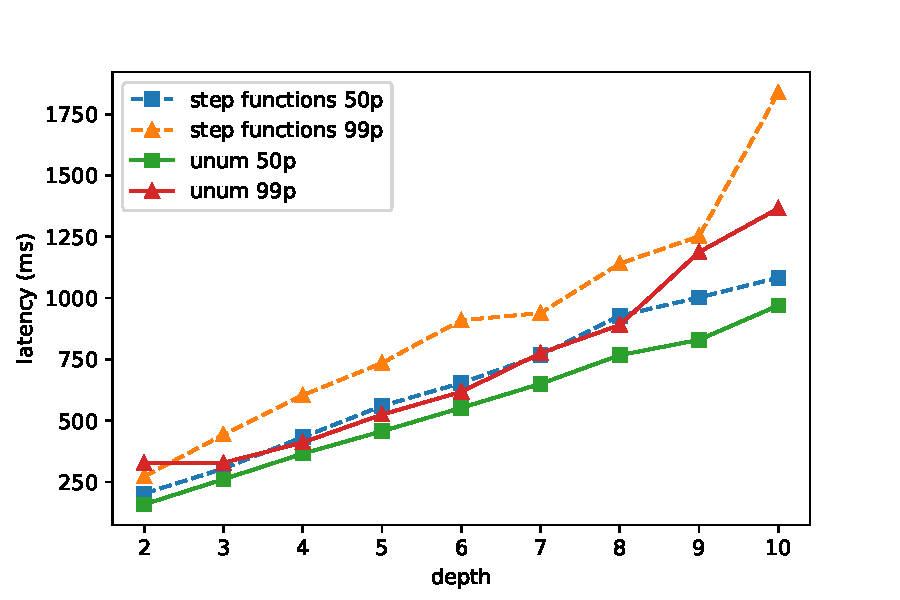
\includegraphics[width=\columnwidth]{figures/ChainMicroLatency.pdf}
    \caption{End-to-end latency of chaining N functions. All constituent
    functions in the experiment only run for 1-2ms, so the results mostly
    reflect the latency of the workflow systems. \name{} is marginally
    (11-28\%) faster than Step Functions on average. The results show that
    \name{} is basically as fast in the most fundamental orchestration
    primitive of transitioning from one function to the next.}
    \label{fig:chainmicrolatency}
\end{figure}

\begin{figure}[t!]
    \centering
    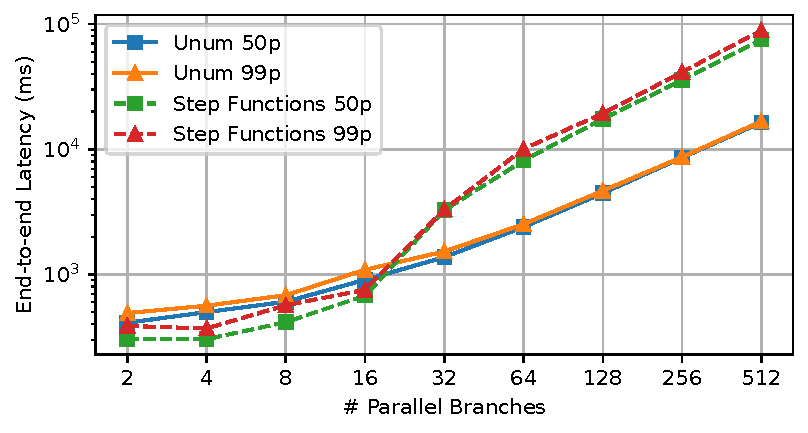
\includegraphics[width=\columnwidth]{figures/MapMicroLatency.pdf}
    \caption{End-to-end latency of parallel fan-out and fan-in with varying
    degrees of parallelism. All constituent functions in the experiment only
    run for 1-2ms, so the results mostly reflect the latency of the workflow
    systems. \name{} is around 100-200ms slower at lower degrees of
    parallelism (2-16 parallel branches), but starts to outperform Step
    Functions (2.37x faster) at even moderate parallelism level of 32 parallel
    branches. \name{}'s advantage widens as the the degress of parallelism
    increases, and is up to 4.58x at 512 parallel branches.}
    \label{fig:mapmicrolatency}
\end{figure}

\subsubsection{Chaining performance}\label{sec:eval:chain}

In this section, we discuss how \name{} performs on executing a series of step
in sequence, using the basic \texttt{chain} pattern, and compares with Step
Functions. We measure the end-to-end latency of executing a chain of functions
with varying chain length (2 to 10 functions). We want the end-to-end latency
to maximally reflects the performance of the workflow system, and not the
latency of user code. Therefore, we use a constituent function that simply
returns its input without any computations to keep the user code runtime
intentionally short (less than 2ms).

Figure~\ref{fig:chainmicrolatency} shows the end-to-end latency of Step
Functions and \name{} with DynamoDB. Overall, \name{} is around 43-173ms or
11-28\% faster in chaining than Step Functions. The slighly shorter latency is
likely because a transition in \name{} from one function to the next involves
a single network communication to Lambda when the source function calls the
target function asynchronously. On the other hand, in a centralized
orchestrator, the same transition first requires a network communication from
the source function to the orchestrator to send back the function output and
then an invocation from the orchestrator to Lambda. \name{} reduces the number
of network communications because control-flow states and logic are
decentralized to constituent functions and not managed by a centralized
orchestrator.

\subsubsection{Single Transition Performance}

Using the same experiment from the last section, we further breakdown the
latency for a single transition from one function to the next.

\subsubsection{Fan-out and fan-in performance}\label{sec:eval:fan-out}

Next, we evaluate another critical orchestration primitive: fan-out and
fan-in. Quickly creating parallel instances is an important operation for
serverless because many applications migrate to serverless for its faster
scalability.

Step Functions has two state types, \texttt{Map} and \texttt{Parallel}, for creating
parallel branches. \name{} supports both. This microbenchmark uses the
\texttt{Map} state because it allows easy control on the number of parallel
branches.

Similarly, we use a function that simply returns its input without any
computations in this microbenchmark to minimize the runtime of user code so
that the end-to-end latency maximally reflects the performance of the workflow
system. \shadi{do we have any benchmarks with growing amount of computation in the function itself?  or  a few representative datapoints.}

Figure~\ref{fig:mapmicrolatency} shows the end-to-end latency (logscale) of
fan-out and fan-in at varying levels of parallelism. At lower level of
parallelism (2-16 parallel branches), \name{} is around 100-200ms slower than
Step Functions. \shadi{what \% is this?} \name{} starts to outperform Step Functions at even moderate parallelism level of 32
parallel branches (2.37x) and up to 4.58x at 512 parallel branches. \shadi{is it common to have >32 parallelism?}

As we do not have direct access to Step Functions's backend, it is difficult to
understand why Step Functions's performance becomes worse at higher parallelism. One
possible cause of higher latency is throttlng of concurrent branch creations.
Step Functions documentation states that it might pause creating branches when the
fan-out size exceeds 40~\cite{aws-step-functions-map-state}.

Our result is not arguing that orchestrator-based workflow systems
fundamentally scales worse than \name{}. Although Step Functions does not
elaborate on the reason for throttling, there is little reason to believe that
the maximum allowable concurrency must be capped around 40 for parallel
workloads.

However, this result does demonstrate an important downside of relying on
supplemental services to support serverless workflows. Any services added must
also perform well compared with the highly scalable FaaS engine, otherwise
application developers have to work with the restrictions that the services
impose. \name{} avoids the difficulty of building and maintaining hosted
orchestrators and directly leverages the scalability of Lambda to achieve
better parallel performance.

\begin{figure}[t!]
    \centering
    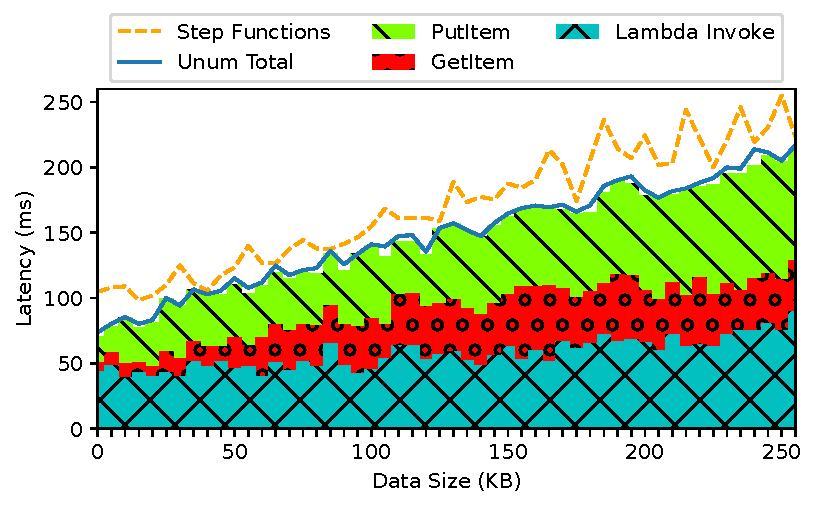
\includegraphics[width=\columnwidth]{figures/TotalAdditionalLatencyNBreakdown.pdf}
    \caption{\name{} latency of transitioning from the completion of a funtion
    to the start of the next function. The transition involves a Lambda
    invoke call, a checkpoint write to data store (a DynamoDB PutItem call)
    and a checkpoint read from data store (a DynamoDB GetItem call). Overall
    latency increases with data size due to more data written in the PutItem
    call and sent to next function via the Lambda invoke call. Over 97.5\% of
    the latency is the
    \name{} runtime waiting for data store accesses and Lambda invoke API
    calls to return. When the underlying platform improves (e.g., a faster
    Lambda or data store), the bulk of \name{}'s performance will
    automatically improve without any modification to \name{} itself.}
    \label{fig:totallatency}
\end{figure}

\subsubsection{Single transition performance}

A fundamental operation of any serverless workflow system is the transition
between a function's completion and the next function's start. The latency
of transitions bounds the end-to-end performance of workflows. In \name{},
this transition involves (1). writing a checkpoint, (2). invoking the
continuation, and (3). reading a checkpoint. That is two storage accesses and
at least one Lambda \texttt{invoke} call.

Therefore, we start our evaluation by measuring the latency of a single
transition and further breaking it down into the latencies of the Lambda
\texttt{invoke} and data store read and write API calls.

The microbenchmark we use is a chain of two functions (\texttt{F->G}) that
simply return their input without performing any computations. Invoking the
continuation involves a single call to the Lambda \texttt{invoke} API.

Because the latency of storage accesses and the Lambda \texttt{invoke} APIs
depend on how much data is written to the checkpoint and then sent to the next
function as the invocation payload, we measure across data sizes ranging
between 0-255KB in 5KB increments\footnote{Lambda limits payload size to 256KB
for async invocations.}.

As a baseline, we also measure the same latency of a state transition in Step
Functions. However, Step Functions does not generate fine-grained enough logs
for us to measure the exact apple-to-apple comparison. The results we show
measure between a \texttt{LambdaFunctionSucceeded} event and the next
\texttt{LambdaFunctionStarted} event. This is likely an underestimate because
it may not include the latency of persisting function outputs. In fact, based
on end-to-end performance of chaining (Figure~\ref{fig:chainmicrolatency}), it
is almost certain that we are not measuring all of the latency in a state
transition.

Figure~\ref{fig:totallatency} shows the total latency of a transition. \name{}
incurs 73-217ms of latency, depending on the data size. A likely underestimate
of Step Functions latency notwithstanding, \name{} is 1.09-3.54x slower than
Step Functions on a single transition. \shadi{can you show step function latency in  figure 6.  Also, if the number is not representative, why do we mention it? it seems misguiding. being 3.5x slower is not good... maybe just say we cannot measure transitions for step functions, and instead we compare the e2e latency.  }

Figure~\ref{fig:oplatency} shows the latency of the Lambda \texttt{invoke}
API, the DynamoDB \texttt{GetItem} call to read a checkpoint and the DynamoDB
\texttt{PutItem} call to write a checkpoint. Overall, all three operations
slows down as data size increases.

Figure~\ref{fig:oplatency-pct} shows the latency breakdown for 0KB data size
and 255KB data size. Over 97.5\% of the latency comes from APIs call to Lambda
and data stores. \name{} runtime code only incurs less than 2.5\% of the total
overhead. This means the bulk of \name{}'s performance will automatically
improve with the underlying platform (e.g., a faster Lambda or data store)
without any modification to \name{} itself.

\subsubsection{Cost comparison}

\begin{figure}[t!]
    \centering
    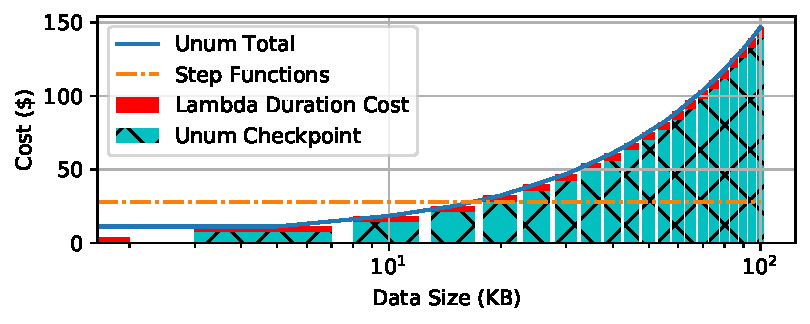
\includegraphics[width=\columnwidth]{figures/TotalCost.pdf}
    \caption{Total costs comparison of 1 million state transitions between
    Step Functions and \name{}. Computation assumes Lambda size of 3GB. \shadi{colors are hard to read}}
    \label{fig:total-costs-single}
\end{figure}

\begin{figure}[t!]
    \centering
    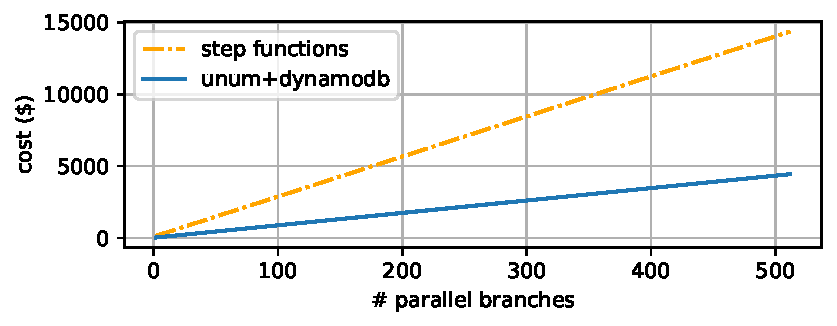
\includegraphics[width=\columnwidth]{figures/TotalMapCost.pdf}
    \caption{Total costs comparison of fan-out and fan-in between Step
    Functions and \name{}. Computation assumes Lambda size of 3GB and 1KB data
    size for function outputs and checkpoints.}
    \label{fig:total-costs-map}
\end{figure}



In this section, we break down the cost of running workflows with \name{} and
compare with that of Step Functions. We discuss the costs for a single transition,
chaining and fan-out.

Costs numbers are calculated based on AWS pricing for \texttt{us-west-1}
region. We do not "measure" the cost of running workflows because AWS does not
provide real-time billing data. We scale costs numbers by 1 million to ease
reading.

Step Functions charges based on the number of state
transitions~\cite{aws-step-functions-pricing}. Each state transition is charged
a fixed rate of \$27.9 $ \times 10^{-6}$.

There are two parts to \name{}'s costs: (1). additional Lambda duration
billing for running the \name{} runtime, and (2). data store reads and writes.

We do not count the storage costs in the intermediary data store because after
a workflow execution, checkpoints can be immediately deleted or moved to
cheaper storage by the user.

Figure~\ref{fig:total-costs-single} shows the total cost of transitions for
function data size varying between 0-255KB. The computation assumes Lambda
memory size of 3GB. We can see that the additional Lambda duration costs from
running \name{} runtime is a small fraction when compared with the costs of
DynamoDB writes. \shadi{how is the figure showing this? how do you translate lambda duration to cost in the figure? this figure is hard to understand. }
In fact, even at 255KB, the additional Lambda
duration costs is only abour \$10. If using the smallest 128MB lambdas \shadi{(instead of 3GB)}, the
costs diminishes to merely \$0.46.

DynamoDB writes dominates the costs in \name{} because the on-demand mode
charges only not on the number of writes but also on the amount of data
written. For 1KB of data, DynamoDB charges $1.3942 \times 10^{-6}$ for a write
and $0.279 \times 10^{-6}$ for a read. Because checkpoint reads do not return
any data when there are no faults, the cost of checkpoint reads does not
increase with the data size and stays merely \$0.279 for the computation in
Figure~\ref{fig:total-costs-single}.

Even though the simulation in Figure~\ref{fig:total-costs-single} shows the
costs of \name{} outpacing that of Step Functions at larger data sizes, our
macrobenchmark results demonstrate that functions in real-world serverless
workflows do not output large amount of data. In fact, workflows tend to use
their own storage and manage application data manually. Checkpoints in the
\name{} intermediary data store are normally under 1KB. \shadi{currently, the graph look very much not in favor of Unum. it seems like a big part of the time, it just works worse. If our argument is that usually data sizes are small, do we have to show such a big range? maybe use a log scale so at least we can focus on the important part of the range?}

Figure~\ref{fig:total-costs-map} shows the total costs of fan-out and fan-in
when function checkpoints are under 1KB. In addition to the costs discussed
for a single transition, the entry function performing the fan-out incurs
higher Lambda duration costs for invoking each fan-out function. The fan-in
function at the end also causes extra costs because it reads the checkpoints
of all fan-out branches. However, the total costs of this microbenchmark is
more than 3.2x lower with \name{} than Step Functions.

% \begin{itemize}

%     \item S3 charges \$5.5 per 1M PUT requests (for checkpoint write) and \$0.44
%     per 1M GET requests (for checkpoint read).

%     \item DynamoDB on-demand capcity mode charges reads and writes based on
%     the data size. 1M requests for writing 1KB data costs \$1.3942 and 1M
%     requests for reading 1KB data costs \$0.279. Note that in the case of
%     DynamoDB, if no faults happen during execution, the checkpoint read will
%     return "item not found", which costs the same as returning 1KB of data.

%     \item For 1M state transitions, \name{}'s costs for S3:

%     \[  r(d)\times0.05 + 5.94 \]

%     and for DynamoDB:

%     \[  r(d)\times0.05 + d\times1.3942 +0.279\],

%     where $r$ is the total additional runtime of \name{}, $d$ is the data
%     size.

% \end{itemize}




\subsection{Real-World Applications}

% \begin{table}[]
% \begin{tabular}{llllll}
% \hline
%                      &                        & \multicolumn{2}{l}{\textbf{unum}}                                                                                                   & \multicolumn{2}{l}{\textbf{Step Functions}}                                                                     \\
% \textbf{Application} & Pattern                & \textit{e2e latency} & \textit{cost (per 1M exec.)}                                                                                 & \textit{e2e latency} & \textit{cost (per 1M exec.)}                                                             \\ \hline
% IoT Pipeline         & chain                  & 120.9ms              & $0.2*2+(73+28)*$0.0021+2*\$1.3942                                                                            & 226.52               & $0.2*2+ 4*$27.9                                                                          \\
% Text Processing      & fan-out, fan-in        & 562.69ms             & $0.2*6+ (105+149+70+68+144+100)*$0.0021 + 6*$1.3942+2*2*$0.279                                               & 552.46ms             & $0.2*5+7*$27.9                                                                           \\
% Wordcount            & chain, fan-out, fan-in & 410s                 & $0.2*(1+262+1+250+1) + (277+6264*262 + 348 + 667*250 +68)*$0.0021 +(1+262+1+250+1)*$1.3942 + 262*2*$0.279+ 250*2* $0.279    & 898s                 & $0.2*(1+262+1+250+1) + (5913*262 + 154 + 633*250 +5)*$0.0021 +(1+262+1+1+250+1+1)*\$27.9 \\
% ExCamera             & chain, fan-out, fold   & 84s                  & $0.2*(1+16+15+15+14) + (6500+1500+350+4500+5000)*$0.0021+ (1+16+15+15+14)*$1.3942 + 15*2*$0.279+14*2*\$0.279 & 98s                  & $0.2*(16+16+1+16+15)+(6300+1400+2+5500+5300)*$0.0021+(1+16+16+1+1+16+1+1)*\$27.9      \\ \hline
% \end{tabular}
% \end{table}

\begin{table*}[t]
\centering
\begin{tabular}{ll|rr|rr}
\hline
                     &                        & \multicolumn{2}{c}{\textbf{\name{}}}            & \multicolumn{2}{c}{\textbf{Step Functions}}       \\
\textbf{Application} & \textbf{Pattern}       & \textit{e2e latency} & \textit{cost (per 1 mil. exec.)}   & \textit{e2e latency} & \textit{cost (per 1 mil. exec.)}            \\ \hline
IoT Pipeline         & chain                  & 0.12s              & \$3.4      & 0.23s       & \$111.6    \\
Text Processing      & fan-out, fan-in        & 0.56s             & \$12.0      & 0.55s        & \$196.3   \\
Wordcount            & chain, fan-out, fan-in & 410.64s                 & \$4,904.8   & 898.56s                 & \$18,113.0 \\
ExCamera             & chain, fan-out, fold   & 84.17s                  & \$150.9 & 98.42s                  & \$1,530.0      \\ \hline
\end{tabular}
\caption{Latency and costs comparison between \name{} and Step Functions for
the macrobenchmark applications. Running applications on \name{} is 3.7x to
32.8x cheaper than on Step Functions. \name{} delivers more than one
order-of-magnitude cost savings for all but wordcount. Furthermore, \name{} is
faster than Step Functions especially for workflows with high degrees of
parallelism. Text Processing is the only workflow which \name{} is marginally
slower because Step Functions creates parallel branches faster at low fan-out
degrees as we illustrated in Figure~\ref{fig:mapmicrolatency}. 
\shadi{suggestion: put all cost into one column (w/ two sub-columns, Unum and SF) and e2e latency in another. It would be easier to compare.}}
\label{table:macro}
\end{table*}

We further evaluate \name{}'s performance, costs and expressiveness with 4
real-world applications. 

\paragraph{IoT Pipeline} Adapted from a humidity control application in the
AWS serverless repository~\cite{iot-pipeline}. The workflow consists of a
chain of two functions that processes climate control data and change the HVAC
setting.

\paragraph{Text Processing} Adapted from the social network application in
DeathStarBench~\cite{deathstar}. The workflow consists of 5 functions that
create a social network post by processing user mentions, shortening URLs and
eventually saving the post in a DynamoDB table.

\paragraph{Wordcount} MapReduce word count~\cite{mapreduce} ran with 250
parallel mappers and reducers.

\paragraph{ExCamera} The ExCamera video encoder~\cite{excamera, gg-atc}. We
use the same workload and setup as the experiment in gg~\cite{gg-atc}: the same
input video of the first 888 chunks of sintel 4K, 3GB lambdas and 16 chunks
per batch.

Table~\ref{table:macro} lists the median end-to-end latency and computed costs
per 1 million executions. Both latency and costs numbers are based on DynamoDB
as the intermediary data store. \name{} is slower than Step Functions for Text
Processing where the workflow fans out to 2 parallel branches. \shadi{it is only marginally slower. Maybe we don't want to give the impression that we are slow at low parallelism.} However,
\name{} is faster in the other applications that consists of chaining and
fan-outs at much higher level of parallelism.

Furthermore, \name{} is consistently cheaper than Step Functions for all
workloads with 3.7x to 32.8x costs savings. Most applications manually manage
application data with their own storage and function checkpoints are smaller
than 1KB for all 4 workflows.

\subsubsection{ExCamera}\label{sec:eval-excamera}

\begin{itemize}

    \item \name{} is able to express and execute parallel pipelines while Step
    Functions has to serialize the decode and re-encode stages.

    \item Step Functions does not have a way to express fold, so the last
    rebase stage has to be written as a single recursive function. \name{}
    supports fold. The recursion logic is lifted to the \name{} IR and the
    rebase function is written similarly to ExCamera.

    \item \name{} is 7.1\% faster than gg's implementation of ExCamera and
    \%10.5 slower than the original ExCamera. Similar to gg, \name{} also do
    not pre-load the input data from S3. Different from gg, \name{} does not
    use a long-running coordinator on EC2 to manage communications and
    invocations.

\end{itemize}

% \subsubsection{Questions}

% \begin{enumerate}

%     \item How do we evaluate and present execution guarantee? Anything to show
%      to convince our reader that it's correct?

%     \item How do we evaluate other benefits that stem from a simpler design
%      (the fact that unum gets rid of the needs for a separate orchestrator
%      service), such as resource management, required staffing and other
%      hosting costs? Further on the resource utilization point, do we want to
%      say that dollar costs of running applications is a reasonable enough
%      proxy to resource consumption and therefore lower price = less resource
%      consumption = better resource utilization?

%     \item Should we run experiments with S3 and present those numbers?

%     \item How to discuss the expressiveness advantage? Specifically,

%         Step Functions has no way to express a for loop or fold.

%         Step Functions has no way to express pipeline parallelism.

%         Step Functions fan-in needs to make sure the aggregate data doesn't exceed a
%         limit, unum automatically passes data in using pointers to the intermediary
%         data store.

% \end{enumerate}

